\documentclass{article}
\usepackage{amsmath, amsthm}
\usepackage{listings, xcolor}
\usepackage{graphicx}
\usepackage[pdfborder=000]{hyperref}

\title{Report to Project-3}
\author{Yuanbo Han\quad15300180032}
\date{December 10, 2017}

\graphicspath{{figures/}}

\lstset{
columns=fixed,
numbers=left,
frame=none,
keywordstyle=\color[RGB]{40,40,255},
numberstyle=\footnotesize\color{darkgray},
commentstyle=\it\color[RGB]{0,96,96},
stringstyle=\rmfamily\slshape\color[RGB]{128,0,0},
showstringspaces=false,
language=Matlab,
}

\begin{document}
\maketitle

\tableofcontents

\section{Implements}
\subsection{Determine $nHidden$}
\label{sec-1.1}
When it comes to a neural network model, we always have to decide the network structure, i.e. the number of layers and of hidden units in each layer. Unfortunately, there are currently no theoretical or rigorous methods for determining them. But some empirical summaries and formulae do work well in practice. One experience is that, in MLP, we usually set only one hidden layer, as long as the number of features is not fairly large. Since here we have 256 features for each observed data, the network would contain no more than 2 hidden layers. And I will check it soon that only 1 hidden layer is enough.

Another useful formula is $\frac{2}{3} \times (features + labels)$. This is often a good number of hidden units with single hidden layer for MLP. In this question, $\frac{2}{3} \times (256 + 10) \approx 177$. 

During experiment, I adopt one hidden layer. Surprisingly, I find it workable to plot the average validation error of 10 runs, against the number of hidden units, for the network is not so complicated. I write the script \emph{plotnHidden.m} to plot \hyperref[fig-1]{Figure~1}. Note that the function \emph{MLPclassificationLoss\_mat} applied in the script is the optimized function in \hyperref[sec-1.3]{Section~1.3}, which does the same thing as but is much faster than the original function \emph{MLPclassificationLoss}.

From \hyperref[fig-1]{Figure~1}, we shall take $nHidden = [120]$. The validation error is now around $24\%$. 

\begin{verbatim}
Training iteration = 9500, validation error = 0.245400
Test error with final model = 0.227000
Elapsed time is 7.681454 seconds.
\end{verbatim}

In the following sections, we \textbf{always} set $nHidden = [120]$, because this is part of the basic parameters of a neural network model.

\begin{figure}
	\centering
	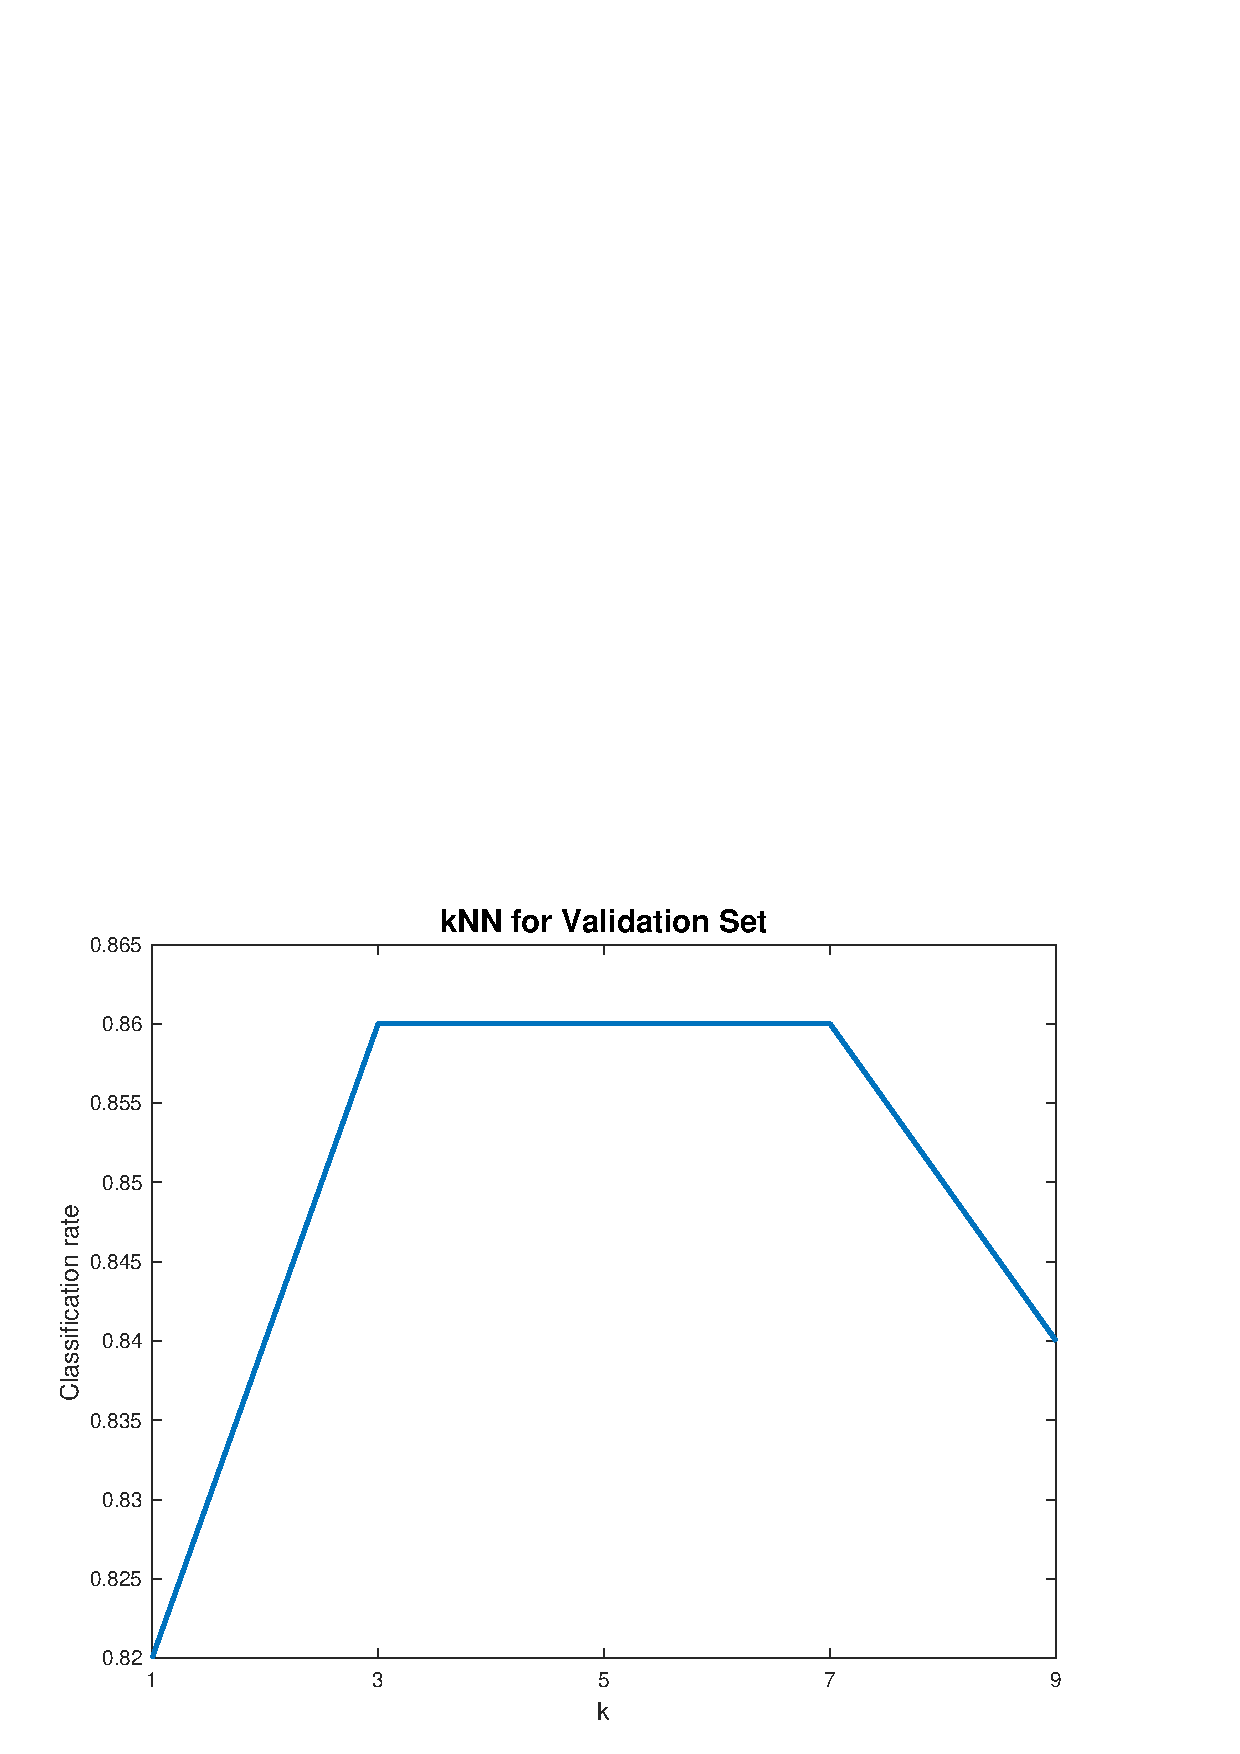
\includegraphics[scale=0.3]{1.png}
	\caption{Validation error against $nHidden$}
	\label{fig-1}
\end{figure}

\subsection{Step Size and Momentum}
\subsubsection{Step Size}
A big step size at early stage could effectively accelerate the learning process, whereas a small one usually results in an accurate convergence. So we make the step size decreases as the training processes.
\[
stepSize = max\_stepSize - \frac{iter}{maxIter} (max\_stepSize - min\_stepSize)
\]
Implement in codes: \\
$\cdots$
\begin{lstlisting}
max_stepSize = 1e-3 * 5;
min_stepSize = 1e-4 * 5;
\end{lstlisting}
$\cdots$
\begin{lstlisting}
stepSize = max_stepSize - iter/maxIter * (max_stepSize - min_stepSize);
w = w - stepSize * g;
\end{lstlisting}
$\cdots$

\subsubsection{Momentum}
Add a momentum via modifying a small part of codes when updating $Weights$: \\
$\cdots$
\begin{lstlisting}
stepSize = 1e-3 * 3;
momentumStrength = 0.9;
delta = 0;
\end{lstlisting}
$\cdots$
\begin{lstlisting}
    [~,g] = funObj(w,i);
    delta = stepSize * g - momentumStrength * delta;
    w = w - delta;
\end{lstlisting}
$\cdots$

By adding a momentum, we could set the initial $stepSize$ bigger, which helps accelerating the learning process but not result in vibration meanwhile. To its credit, there is high chance that the potential vibration around target is avoided.

\begin{verbatim}
Training iteration = 9500, validation error = 0.269800
Test error with final model = 0.259000
Elapsed time is 7.603368 seconds.
\end{verbatim}

As we see, with enough iteration, adding a momentum does not improve the final performance of our model. However, if we check the intermediate steps, we shall find that it usually takes only around 4000 iterations to reach $30\%$ validation error, whereas the original model (used in \hyperref[sec-1.1]{Section~1.1}) need to learn 6000 or so times.

In conclusion, adding a momentum increases the speed of converging, but usually cannot improve accuracy.

\subsection{Optimize Program}
\label{sec-1.3}
The new function \emph{MLPclassificationLoss\_mat} written by me has approximately tripled the programming efficiency. Every thing has been tried best to operate by matrix. Not a detail is left for whether a single hidden layer or multiple hidden layers. Even when $nargout == 1$, or rather, when we only need to compute the squared-error, the program is accelerated. On the other hand, I also made small fixes on function \emph{MLPclassificationPredict} by defining variables before assignment.

Before optimization:
\begin{verbatim}
Training iteration = 9500, validation error = 0.262400
Test error with final model = 0.236000
Elapsed time is 16.313542 seconds.
\end{verbatim}

After optimization:
\begin{verbatim}
Training iteration = 9500, validation error = 0.240600
Test error with final model = 0.254000
Elapsed time is 6.403858 seconds.
\end{verbatim}

\subsection{L2-Regularization}
Regularization, especially L2-regularization, is a common proposal to avoid overfitting in learning models. To be specific, $E = E_0 + \frac{\lambda}{2} ||w||_2^2$, where $E_0$ is the original error. Don't forget there is a trick that the bias need not be regularized. I write function \emph{MLP\_L2} to add L2-regularization of $Weights$ to the loss function.

Having completed the preparation, we are ready to select $\lambda$. \emph{plotLambda.m} written by me plots how the average validation error of 10 runs changes as $\lambda$ increases from $0.001$ to $0.512$ (See \hyperref[fig-2]{Figure~2}).

\begin{figure}
	\centering
	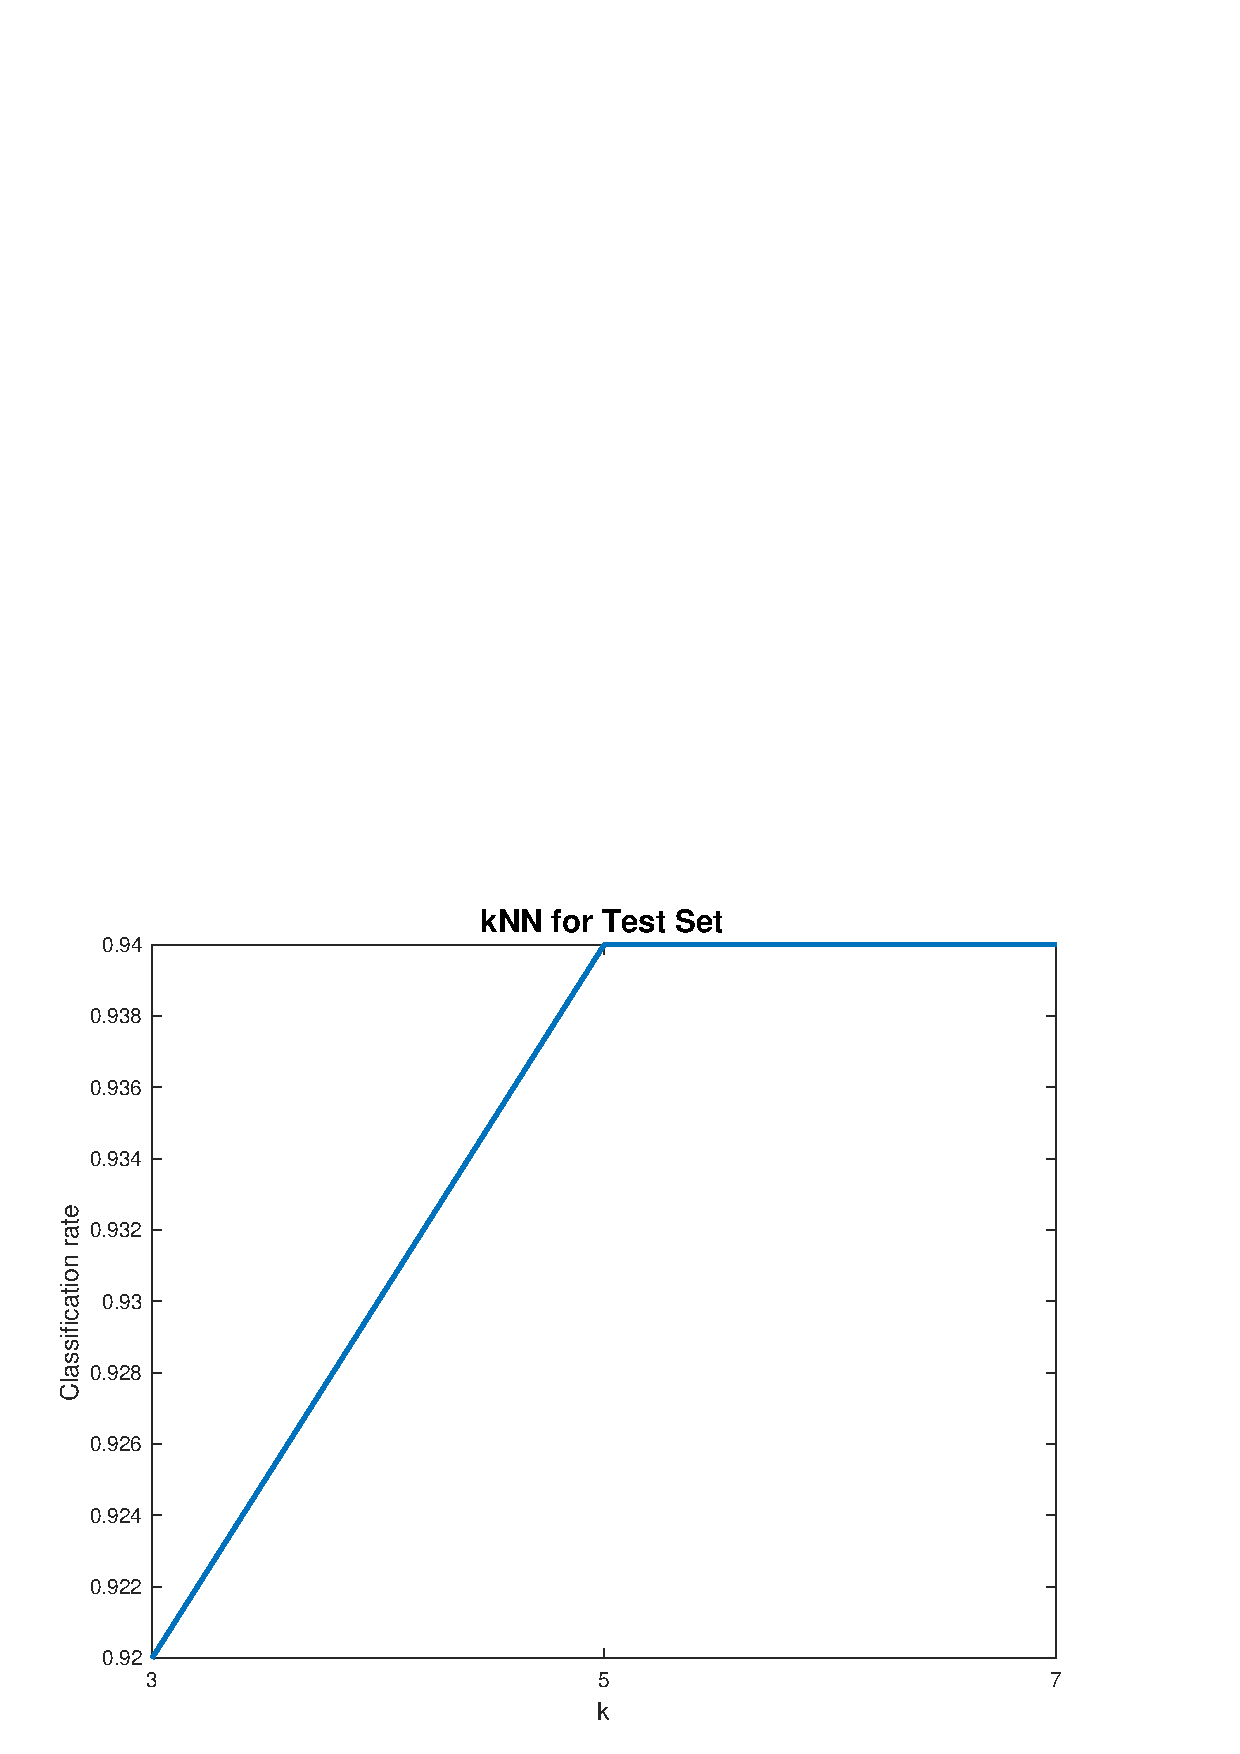
\includegraphics[scale=0.3]{2.png}
	\caption{Validation error against $\lambda$}
	\label{fig-2}
\end{figure}

Obviously, $\lambda \approx 0.03$ performs best. Let's set $\lambda = 0.03$ and iterate 100000 times. The validation error is about $5\%$. L2-regularization largely improves the model!

\begin{verbatim}
Training iteration = 95000, validation error = 0.056600
Test error with final model = 0.049000
Elapsed time is 42.722980 seconds.
\end{verbatim}

\subsection{Softmax}
The softmax function is defined as
\[
p(y_i) = \frac{\exp(z_i)}{\sum_{i=j}^J \exp(z_j)}
\]
Use the cross entropy as the loss function instead of squared-error:
\[
L = -\log p(y_t)
\]
where $t$ is the true label.

Now consider $\frac{\partial L}{\partial z_i}$. When $i = t$,
\begin{align*}
\frac{\partial L}{\partial z_t} &= \frac{\partial L}{\partial p(y_t)} \frac{\partial p(y_t)}{\partial z_t} \\
&= -\frac{1}{p(y_t)} \left( p(y_t) - p(y_t)^2 \right) \\
&= p(y_t) -1
\end{align*}
when $i \ne t$,
\begin{align*}
\frac{\partial L}{\partial z_i} &= \frac{\partial L}{\partial p(y_t)} \frac{\partial p(y_t)}{\partial z_i} \\
&= -\frac{1}{p(y_t)} \left( -p(y_t) p(y_i) \right) \\
&= p(y_i)
\end{align*}

Based on these, I write function \emph{MLP\_softmax} to compute the gradients of $Weights$. The validation error with 100000 iterations is about $20\%$.

\subsection{Add Bias}
As we can imagine, the value (before $tanh$) of a hidden unit might not be completely a linear form of its inputs. In most cases, there do exist a bias, so we shall add them up. I write function \emph{MLP\_addbias} to make one of the hidden units in each layer a constant, so that each layer has a bias. Note that with as we changed the network structure, the predicting function should also be modified. Use \emph{MLP\_addbias\_predict} instead of \emph{MLPclassificationPredict}, and the whole script is modified as \emph{addBias6.m}.

Running it once, the result is below:
\begin{verbatim}
Training iteration = 9500, validation error = 0.246000
Test error with final model = 0.248000
Elapsed time is 6.076616 seconds.
\end{verbatim}

\subsection{Dropout}
The dropout method is widely applied to complicated networks in case of overfitting. To carry it out, we multiply each hidden units an independent $\mathrm{Bernoulli}(1-p)$-distributed random variable, where $p$ is exactly the probability of dropping out. The implementing function is \emph{MLP\_dropout}.

Setting $p=0.5$, the results are below:
\begin{verbatim}
Training iteration = 9500, validation error = 0.233800
Test error with final model = 0.224000
Elapsed time is 6.450364 seconds.
\end{verbatim}

As a result, the model has not been improved evidently. This is probably because our network is such an elementary topology that adopting dropout is needless.

\subsection{Fine-tune by Least Squares}
The error we are using is actually the $residual sum of squares (RSS)$ defined by $||\hat{y} - y||_2^2$. In Project-1, we have already discussed that for $y = XW$, when $RSS$ reaches its minimal,
\begin{equation}
W = \left( X^T X \right)^\dagger X^T y \tag{$\ast$} \label{equ-RSS}
\end{equation}
where $\left( X^T X \right)^\dagger$ is the Moore-Penrose pseudoinverse of $X^T X$.
Therefore, for $outputWeights$, we could alternatively compute them by $\eqref{equ-RSS}$.

My function \emph{MLP\_finetune} first overwrite $outputWeights$ by $\eqref{equ-RSS}$, and then computes the gradients as \emph{MLPclassificationLoss\_mat} does. It also returns the new $w$ besides $f$ and $g$.

Iterating 10000 times, the results turn out to be:
\begin{verbatim}
Training iteration = 9500, validation error = 0.841800
Test error with final model = 0.873000
Elapsed time is 23.957619 seconds.
\end{verbatim}

An awfully poor performance! Why? Because what we are adopting is the best $outputWeights$ for only one sample from training set. Such being the case, We are unlikely to assume they work well for any other observation. From my perspective, this method to determine $outputWeights$ should only be implemented for the first training. In other words, Initialize $outputWeights$ by $\eqref{equ-RSS}$. Then do stochastic gradient descend as usual, and \textbf{never} compute $\eqref{equ-RSS}$ \textbf{again}.

\subsection{Image Transformation}
One can write numbers at different positions, in various sizes, and slantly or straightly. Considering these situation, we could artificially create more training examples, by applying small transformations (translations, rotations, resizing, etc.) to the original images.

Script \emph{creattrain.m} enlarges the training set 9 times. Each original image is respectively translated 1 pixel right, left, down, up, and rotated 5 degree clockwise, anti-clockwise, and resized 10\% larger, smaller. Built-in functions \emph{imtranslate}, \emph{imrotate} and \emph{imresize} are used.

The results for 10000 iterations are:
\begin{verbatim}
Training iteration = 9500, validation error = 0.277000
Test error with final model = 0.261000
Elapsed time is 4.983946 seconds.
\end{verbatim}

\subsection{CNN}
In this section, we will add a 2D convolutional layer between input and hidden layer.
\emph{convol10.m} is my main script carrying this out. Three of my functions are involved in total.

\emph{convolution\_f} computes the full-connected-layer values.

\emph{CNN\_update} computes the gradients of weights, kernels and bias, and then updates these parameters by stepSize using gradient descent method.

\emph{CNN\_predict} classifies samples by the current CNN model.

Since I have written adequate comments step by step in the script and functions (See \hyperref[code-10]{A.15}), there is no need to analyze the detail again.

Running \emph{convol10.m}, the results are:
\begin{verbatim}
>> convol10
Training iteration = 0, validation error = 0.922600
Elapsed time is 38.988072 seconds.
Training iteration = 10000, validation error = 0.231400
Elapsed time is 292.766576 seconds.
Training iteration = 20000, validation error = 0.205400
Elapsed time is 291.313784 seconds.
Training iteration = 30000, validation error = 0.206000
Elapsed time is 299.403606 seconds.
Training iteration = 40000, validation error = 0.182800
Elapsed time is 292.518354 seconds.
Training iteration = 50000, validation error = 0.191600
Elapsed time is 290.924409 seconds.
Training iteration = 60000, validation error = 0.189600
Elapsed time is 299.459586 seconds.
Training iteration = 70000, validation error = 0.180000
Elapsed time is 324.002883 seconds.
Training iteration = 80000, validation error = 0.178600
Elapsed time is 316.184651 seconds.
Training iteration = 90000, validation error = 0.170400
Elapsed time is 315.688232 seconds.
Training iteration = 100000, validation error = 0.169400
Test error with final model = 0.163000
Elapsed time is 283.742722 seconds.
\end{verbatim}

The model has been improved a lot. However, the learning processes quite slow.

\section{My Model}
My final model uses single hidden layer with 120 units, and applies methods in Section~1.4 with $\lambda = 0.03$, Section~1.6 and Section~1.5. The implement function is \emph{MLP\_softmax\_L2}.

The final test error is about $4\%$.

\appendix
\section{MATLAB Codes}
\subsection{\emph{example\_neuralNetwork.m}}
\begin{lstlisting}
load digits.mat
[n,d] = size(X);
nLabels = max(y);
yExpanded = linearInd2Binary(y,nLabels);
t = size(Xvalid,1);
t2 = size(Xtest,1);

% Standardize columns and add bias
[X,mu,sigma] = standardizeCols(X);
X = [ones(n,1) X];
d = d + 1;

% Make sure to apply the same transformation to the validation/test data
Xvalid = standardizeCols(Xvalid,mu,sigma);
Xvalid = [ones(t,1) Xvalid];
Xtest = standardizeCols(Xtest,mu,sigma);
Xtest = [ones(t2,1) Xtest];

% Choose network structure
nHidden = [120];

% Count number of parameters and initialize weights 'w'
nParams = d*nHidden(1);
for h = 2:length(nHidden)
    nParams = nParams+nHidden(h-1)*nHidden(h);
end
nParams = nParams+nHidden(end)*nLabels;
w = randn(nParams,1);

% Train with stochastic gradient
maxIter = 10000;
stepSize = 1e-3; %* 3;
%momentumStrength = 0.9;
%delta = 0;
%lambda = 0.03;
%p = 0.5;
funObj = @(w,i)MLP_softmax(w, X(i,:), yExpanded(i,:), ...
    nHidden, nLabels);

tic
for iter = 1:maxIter
    if mod(iter-1,round(maxIter/20)) == 0
        yhat = MLPclassificationPredict(w,Xvalid,nHidden,nLabels);
        fprintf('Training iteration = %d, validation error = %f\n', ...
            iter-1, sum(yhat~=yvalid)/t);
    end
    
    i = ceil(rand*n);
    [~,g] = funObj(w,i);
    %delta = stepSize * g - momentumStrength * delta;
    %w = w - delta;
    w = w - stepSize * g;
end

% Evaluate test error
yhat = MLPclassificationPredict(w,Xtest,nHidden,nLabels);
fprintf('Test error with final model = %f\n',sum(yhat~=ytest)/t2);
toc
\end{lstlisting}

\subsection{\emph{plotnHidden.m}}
\begin{lstlisting}
% Edited by Yuanbo Han, Dec. 7, 2017.

load digits.mat;
[n,d] = size(X);
nLabels = max(y);
yExpanded = linearInd2Binary(y,nLabels);
t = size(Xvalid,1);

% Standardize columns and add bias
[X,mu,sigma] = standardizeCols(X);
X = [ones(n,1) X];
d = d + 1;

% Apply the same transformation to the validation data
Xvalid = standardizeCols(Xvalid,mu,sigma);
Xvalid = [ones(t,1) Xvalid];

maxIter = 10000;
stepSize = 1e-3;
validError = zeros(1,40);
% Choose network structure
for nHidden = 5:5:200
    tic
    % Count number of parameters
    nParams = d*nHidden(1);
    for h = 2:length(nHidden)
        nParams = nParams+nHidden(h-1)*nHidden(h);
    end
    nParams = nParams+nHidden(end)*nLabels;
    
    for k = 1:10
        % Initialize weights 'w'
        w = randn(nParams,1);
        
        % Train with stochastic gradient
        funObj = @(w,i)MLPclassificationLoss_mat(w, X(i,:), ...
            yExpanded(i,:), nHidden, nLabels);
        for iter = 1:maxIter
            i = ceil(rand*n);
            [~,g] = funObj(w,i);
            w = w - stepSize*g;
        end
        
        % Evaluate validation error
        yhat = MLPclassificationPredict(w,Xvalid,nHidden,nLabels);
        validError(nHidden/5) = validError(nHidden/5) + ...
            1/10 * sum(yhat~=yvalid)/t;
    end
    fprintf('nHidden = %d\n', nHidden);
    fprintf('Average validation error = %f\n', validError(nHidden/5));
    toc
end

figure;
plot(5:5:200, validError);
xlabel('nHidden', 'FontSize', 12);
ylabel('Validation Error', 'FontSize', 12);
title('Single Hidden Layer', 'FontSize', 14);
\end{lstlisting}

\subsection{\emph{MLPclassificationLoss\_mat.m}}
\begin{lstlisting}
function [f,g] = MLPclassificationLoss_mat(w,X,y,nHidden,nLabels)
% MLPCLASSIFICATIONLOSS_MAT does the same thing as MLPclassificationLoss,
% but computes as much by matrix as possible, which is very fast.
%
% Yuanbo Han, Dec. 5, 2017.

[nInstances, nVars] = size(X);
nHiddenLayers = length(nHidden);

% Form Weights
inputWeights = reshape(w(1:nVars*nHidden(1)),nVars,nHidden(1));
offset = nVars * nHidden(1);
hiddenWeights = cell(1, nHiddenLayers-1);
for h = 2:nHiddenLayers
hiddenWeights{h-1} = reshape(...
w(offset+1:offset+nHidden(h-1)*nHidden(h)),...
nHidden(h-1), nHidden(h));
offset = offset + nHidden(h-1) * nHidden(h);
end
outputWeights = w(offset+1:offset+nHidden(end)*nLabels);
outputWeights = reshape(outputWeights, nHidden(end), nLabels);

ip = cell(1, nHiddenLayers);
fp = cell(1, nHiddenLayers);
if nargout > 1
% Form Gradient
gInput = zeros(size(inputWeights));
gHidden = cell(1, nHiddenLayers-1);
for h = 2:nHiddenLayers
gHidden{h-1} = zeros(size(hiddenWeights{h-1}));
end
gOutput = zeros(size(outputWeights));

f = 0;

% Compute Output
for i = 1:nInstances
ip{1} = X(i,:) * inputWeights;
fp{1} = tanh(ip{1});
for h = 2:length(nHidden)
ip{h} = fp{h-1} * hiddenWeights{h-1};
fp{h} = tanh(ip{h});
end
yhat = fp{end} * outputWeights;

relativeErr = yhat - y(i,:);
f = f + sum(relativeErr.^2);

err = 2 * relativeErr;

% Output Weights
gOutput = gOutput + fp{end}' * err;

if nHiddenLayers > 1
% Last Layer of Hidden Weights
backprop = (err' * sech(ip{end}).^2) .* outputWeights';
backprop = sum(backprop,1);
gHidden{end} = gHidden{end} + fp{end-1}' * backprop;

% Other Hidden Layers
for h = nHiddenLayers-2:-1:1
backprop = (backprop * hiddenWeights{h+1}') .* ...
sech(ip{h+1}).^2;
gHidden{h} = gHidden{h} + fp{h}' * backprop;
end

% Input Weights
backprop = (backprop * hiddenWeights{1}') .* sech(ip{1}).^2;
gInput = gInput + X(i,:)' * backprop;

else % nHiddenLayers == 1
% Input Weights
gInput = gInput + X(i,:)' * ...
( sech(ip{end}).^2 .* (outputWeights * err')' );
end
end

% Put Gradient into vector
g = zeros(size(w));
g(1:nVars*nHidden(1)) = gInput(:);
offset = nVars*nHidden(1);
for h = 2:nHiddenLayers
g(offset+1:offset+nHidden(h-1)*nHidden(h)) = gHidden{h-1};
offset = offset+nHidden(h-1)*nHidden(h);
end
g(offset+1:offset+nHidden(end)*nLabels) = gOutput(:);


else % nargout <= 1
ip{1} = X * inputWeights;
fp{1} = tanh(ip{1});
for h = 2:nHiddenLayers
ip{h} = fp{h-1} * hiddenWeights{h-1};
fp{h} = tanh(ip{h});
end
yhat = fp{end} * outputWeights;

relativeErr = yhat - y;
f = sum(sum(relativeErr.^2));
end

end
\end{lstlisting}

\subsection{\emph{MLPclassificationPredict.m}}
\begin{lstlisting}
function [y] = MLPclassificationPredict(w,X,nHidden,nLabels)
% Modified by Yuanbo Han, Dec. 7, 2017.

[nInstances,nVars] = size(X);
nHiddenLayers = length(nHidden);

% Form Weights
inputWeights = reshape(w(1:nVars*nHidden(1)),nVars,nHidden(1));
offset = nVars*nHidden(1);
for h = 2:nHiddenLayers
hiddenWeights{h-1}=reshape(w(offset+1:...
offset+nHidden(h-1)*nHidden(h)), nHidden(h-1), nHidden(h));
offset = offset+nHidden(h-1)*nHidden(h);
end
outputWeights = w(offset+1:offset+nHidden(end)*nLabels);
outputWeights = reshape(outputWeights,nHidden(end),nLabels);

ip = cell(1, nHiddenLayers);
fp = cell(1, nHiddenLayers);

y = zeros(nInstances, nLabels);
% Compute Output
for i = 1:nInstances
ip{1} = X(i,:)*inputWeights;
fp{1} = tanh(ip{1});
for h = 2:length(nHidden)
ip{h} = fp{h-1}*hiddenWeights{h-1};
fp{h} = tanh(ip{h});
end
y(i,:) = fp{end}*outputWeights;
end
[~, y] = max(y,[],2);
%y = binary2LinearInd(y);
end
\end{lstlisting}

\subsection{\emph{MLP\_L2.m}}
\begin{lstlisting}
function [f,g] = MLP_L2(w,X,y,nHidden,nLabels,lambda)
% MLP_L2 adds L2-regularization of Weights to the loss function.
%
% Yuanbo Han, Dec. 5, 2017.

[nInstances, nVars] = size(X);
nHiddenLayers = length(nHidden);

% Form Weights
inputWeights = reshape(w(1:nVars*nHidden(1)),nVars,nHidden(1));
offset = nVars * nHidden(1);
hiddenWeights = cell(1, nHiddenLayers-1);
for h = 2:nHiddenLayers
hiddenWeights{h-1} = reshape(...
w(offset+1:offset+nHidden(h-1)*nHidden(h)),...
nHidden(h-1), nHidden(h));
offset = offset + nHidden(h-1) * nHidden(h);
end
outputWeights = w(offset+1:offset+nHidden(end)*nLabels);
outputWeights = reshape(outputWeights, nHidden(end), nLabels);

ip = cell(1, nHiddenLayers);
fp = cell(1, nHiddenLayers);
if nargout > 1
% Form Gradient
gInput = zeros(size(inputWeights));
gHidden = cell(1, nHiddenLayers-1);
for h = 2:nHiddenLayers
gHidden{h-1} = zeros(size(hiddenWeights{h-1}));
end
gOutput = zeros(size(outputWeights));

f = 0;

% Compute Output
for i = 1:nInstances
ip{1} = X(i,:) * inputWeights;
fp{1} = tanh(ip{1});
for h = 2:length(nHidden)
ip{h} = fp{h-1} * hiddenWeights{h-1};
fp{h} = tanh(ip{h});
end
yhat = fp{end} * outputWeights;

relativeErr = yhat - y(i,:);
f = f + sum(relativeErr.^2);

err = 2 * relativeErr;

% Output Weights
gOutput = gOutput + fp{end}' * err + lambda * outputWeights;

if nHiddenLayers > 1
% Last Layer of Hidden Weights
backprop = err' * sech(ip{end}).^2 .* outputWeights';
gHidden{end} = gHidden{end} + fp{end-1}' * sum(backprop,1) ...
+  lambda * hiddenWeights{end};

backprop = sum(backprop,1);
% Other Hidden Layers
for h = length(nHidden)-2:-1:1
backprop = (backprop * hiddenWeights{h+1}') .* ...
sech(ip{h+1}).^2;
gHidden{h} = gHidden{h} + fp{h}' * sum(backprop,1) + ...
lambda * hiddenWeights{h};
end

% Input Weights
backprop = (backprop * hiddenWeights{1}') .* sech(ip{1}).^2;
gInput = gInput + X(i,:)' * backprop + lambda * inputWeights;
% The bias need not be included in regularization.
gInput(1,:) = gInput(1,:) - lambda * inputWeights(1,:);

else % nHiddenLayers == 1
% Input Weights
gInput = gInput + X(i,:)' * ...
( sech(ip{end}).^2 .* (outputWeights * err')' ) + ...
lambda * inputWeights;
% The bias need not be included in regularization.
gInput(1,:) = gInput(1,:) - lambda * inputWeights(1,:);
end
end

% Put Gradient into vector
g = zeros(size(w));
g(1:nVars*nHidden(1)) = gInput(:);
offset = nVars*nHidden(1);
for h = 2:nHiddenLayers
g(offset+1:offset+nHidden(h-1)*nHidden(h)) = gHidden{h-1};
offset = offset+nHidden(h-1)*nHidden(h);
end
g(offset+1:offset+nHidden(end)*nLabels) = gOutput(:);


else % nargout <= 1
ip{1} = X * inputWeights;
fp{1} = tanh(ip{1});
for h = 2:nHiddenLayers
ip{h} = fp{h-1} * hiddenWeights{h-1};
fp{h} = tanh(ip{h});
end
yhat = fp{end} * outputWeights;

relativeErr = yhat - y;
f = sum(sum(relativeErr.^2));
end
\end{lstlisting}

\subsection{\emph{plotLambda.m}}
\begin{lstlisting}
% Edited by Yuanbo Han, Dec. 8, 2017.

load digits.mat
[n,d] = size(X);
nLabels = max(y);
yExpanded = linearInd2Binary(y,nLabels);
t = size(Xvalid,1);

% Standardize columns and add bias
[X,mu,sigma] = standardizeCols(X);
X = [ones(n,1) X];
d = d + 1;

% Apply the same transformation to the validation data
Xvalid = standardizeCols(Xvalid,mu,sigma);
Xvalid = [ones(t,1) Xvalid];

% Choose network structure
nHidden = [120];

% Count number of parameters
nParams = d*nHidden(1);
for h = 2:length(nHidden)
nParams = nParams+nHidden(h-1)*nHidden(h);
end
nParams = nParams+nHidden(end)*nLabels;

maxIter = 100000;
stepSize = 1e-3;
funObj = @(w,i,lambda)MLP_L2(w, X(i,:), yExpanded(i,:), nHidden, ...
nLabels, lambda);

lambda = zeros(1,10);
lambda(1) = 0.001;
for i = 2:10
lambda(i) = lambda(i-1) * 2;
end

validError = zeros(1,length(lambda));
for l = 1:length(lambda)
tic
for k = 1:10
% Initialize weights 'w'
w = randn(nParams,1);

% Train with stochastic gradient
for iter = 1:maxIter
i = ceil(rand*n);
[~,g] = funObj(w,i,lambda(l));
w = w - stepSize*g;
end

% Evaluate validation error
yhat = MLPclassificationPredict(w, Xvalid, nHidden, nLabels);
validError(l) = validError(l) + 1/10 * sum(yhat~=yvalid)/t;
end
fprintf('lambda = %.3f\n', lambda(l));
fprintf('Average validation error = %f\n', validError(l));
toc
end

figure;
semilogx(lambda, validError);
set(gca, 'XTick', lambda);
xlabel('\lambda', 'FontSize', 12);
ylabel('Validation Error', 'FontSize', 12);
title('L2-Regularization', 'FontSize', 14);
\end{lstlisting}

\subsection{\emph{MLP\_softmax.m}}
\begin{lstlisting}
function [f,g] = MLP_softmax(w,X,y,nHidden,nLabels)
% MLP_SOFTMAX use a softmax (multinomial logistic) layer at the end of the
% network, and replace squared error with the negative log-likelihood of
% the true label under this loss.
%
% Yuanbo Han, Dec. 8, 2017.

[nInstances, nVars] = size(X);
nHiddenLayers = length(nHidden);

% Form Weights
inputWeights = reshape(w(1:nVars*nHidden(1)),nVars,nHidden(1));
offset = nVars * nHidden(1);
hiddenWeights = cell(1, nHiddenLayers-1);
for h = 2:nHiddenLayers
hiddenWeights{h-1} = reshape(...
w(offset+1:offset+nHidden(h-1)*nHidden(h)),...
nHidden(h-1), nHidden(h));
offset = offset + nHidden(h-1) * nHidden(h);
end
outputWeights = w(offset+1:offset+nHidden(end)*nLabels);
outputWeights = reshape(outputWeights, nHidden(end), nLabels);

ip = cell(1, nHiddenLayers);
fp = cell(1, nHiddenLayers);
f = 0;
% Compute Output
for i = 1:nInstances
ip{1} = X(i,:) * inputWeights;
fp{1} = tanh(ip{1});
for h = 2:length(nHidden)
ip{h} = fp{h-1} * hiddenWeights{h-1};
fp{h} = tanh(ip{h});
end
yhat = fp{end} * outputWeights;
yhat = exp(yhat) / sum(exp(yhat));
yhat_true = (y(i,:)==1) * yhat';

err = -log( yhat_true );
f = f + err;

if nargout > 1
% Form Gradient
gInput = zeros(size(inputWeights));
gHidden = cell(1, nHiddenLayers-1);
for h = 2:nHiddenLayers
gHidden{h-1} = zeros(size(hiddenWeights{h-1}));
end
gOutput = zeros(size(outputWeights));

% Output Weights
gOutput = gOutput - fp{end}' * (1 - yhat_true) * (y(i,:)==1);

% to be modified for nHiddenLayers > 1
if nHiddenLayers > 1
% Last Layer of Hidden Weights
backprop = err' * sech(ip{end}).^2 .* outputWeights';
gHidden{end} = gHidden{end} + fp{end-1}' * sum(backprop,1);

backprop = sum(backprop,1);
% Other Hidden Layers
for h = length(nHidden)-2:-1:1
backprop = (backprop * hiddenWeights{h+1}') .* ...
sech(ip{h+1}).^2;
gHidden{h} = gHidden{h} + fp{h}' * backprop;
end

% Input Weights
backprop = (backprop * hiddenWeights{1}') .* sech(ip{1}).^2;
gInput = gInput + X(i,:)' * backprop;

else % nHiddenLayers == 1
% Input Weights
gInput = gInput - (1 - yhat_true) * X(i,:)' * ...
( sech(ip{end}).^2 .* outputWeights(:, y(i,:)==1)' );
end

% Put Gradient into vector
g = zeros(size(w));
g(1:nVars*nHidden(1)) = gInput(:);
offset = nVars*nHidden(1);
for h = 2:nHiddenLayers
g(offset+1:offset+nHidden(h-1)*nHidden(h)) = gHidden{h-1};
offset = offset+nHidden(h-1)*nHidden(h);
end
g(offset+1:offset+nHidden(end)*nLabels) = gOutput(:);

end
end
end
\end{lstlisting}

\subsection{\emph{addBias6.m}}
\begin{lstlisting}
% Edited by Yuanbo Han, Dec. 8, 2017.

load digits.mat
[n,d] = size(X);
nLabels = max(y);
yExpanded = linearInd2Binary(y,nLabels);
t = size(Xvalid,1);
t2 = size(Xtest,1);

% Standardize columns and add bias
[X,mu,sigma] = standardizeCols(X);
X = [ones(n,1) X];
d = d + 1;

% Apply the same transformation to the validation/test data
Xvalid = standardizeCols(Xvalid,mu,sigma);
Xvalid = [ones(t,1) Xvalid];
Xtest = standardizeCols(Xtest,mu,sigma);
Xtest = [ones(t2,1) Xtest];

% Choose network structure
nHidden = [120];

% Add a constant to each of the hidden layers
% Count number of parameters and initialize weights 'w'
nParams = d*nHidden(1);
for h = 2:length(nHidden)
nParams = nParams+(nHidden(h-1)+1)*nHidden(h);
end
nParams = nParams+(nHidden(end)+1)*nLabels;
w = randn(nParams,1);

% Train with stochastic gradient
maxIter = 10000;
stepSize = 1e-3; %* 3;
%momentumStrength = 0.9;
%delta = 0;
%lambda = 0.03;
funObj = @(w,i)MLP_addbias(w,X(i,:),yExpanded(i,:),nHidden,nLabels);

tic
for iter = 1:maxIter
if mod(iter-1,round(maxIter/20)) == 0
yhat = MLP_addbias_predict(w,Xvalid,nHidden,nLabels);
fprintf('Training iteration = %d, validation error = %f\n', ...
iter-1, sum(yhat~=yvalid)/t);
end

i = ceil(rand*n);
[~,g] = funObj(w,i);
%    delta = stepSize * g - momentumStrength * delta;
%    w = w - delta;
w = w - stepSize * g;
end

% Evaluate test error
yhat = MLP_addbias_predict(w,Xtest,nHidden,nLabels);
fprintf('Test error with final model = %f\n',sum(yhat~=ytest)/t2);
toc
\end{lstlisting}

\subsection{\emph{MLP\_addbias.m}}
\begin{lstlisting}
function [f,g] = MLP_addbias(w,X,y,nHidden,nLabels)
% MLP_ADDBIAS makes one of the hidden units in each layer a constant, so
% that each layer has a bias.
%
% Yuanbo Han, Dec. 8, 2017.

[nInstances, nVars] = size(X);
nHiddenLayers = length(nHidden);

% Form Weights
inputWeights = reshape(w(1:nVars*nHidden(1)),nVars,nHidden(1));
offset = nVars * nHidden(1);
hiddenWeights = cell(1, nHiddenLayers-1);
for h = 2:nHiddenLayers
hiddenWeights{h-1} = reshape(...
w(offset+1:offset+(nHidden(h-1)+1)*nHidden(h)),...
nHidden(h-1)+1, nHidden(h));
offset = offset + (nHidden(h-1) + 1) * nHidden(h);
end
outputWeights = w(offset+1:offset+(nHidden(end)+1)*nLabels);
outputWeights = reshape(outputWeights, nHidden(end)+1, nLabels);

ip = cell(1, nHiddenLayers);
fp = cell(1, nHiddenLayers);
if nargout > 1
% Form Gradient
gInput = zeros(size(inputWeights));
gHidden = cell(1, nHiddenLayers-1);
for h = 2:nHiddenLayers
gHidden{h-1} = zeros(size(hiddenWeights{h-1}));
end
gOutput = zeros(size(outputWeights));

f = 0;

% Compute Output
for i = 1:nInstances
ip{1} = [1, X(i,:)*inputWeights];
fp{1} = tanh(ip{1});
for h = 2:length(nHidden)
ip{h} = [1, fp{h-1}*hiddenWeights{h-1}];
fp{h} = tanh(ip{h});
end
yhat = fp{end} * outputWeights;

relativeErr = yhat - y(i,:);
f = f + sum(relativeErr.^2);

err = 2 * relativeErr;

% Output Weights
gOutput = gOutput + fp{end}' * err;

% to be modified
if nHiddenLayers > 1
% Last Layer of Hidden Weights
backprop = err' * sech(ip{end}).^2 .* outputWeights';
gHidden{end} = gHidden{end} + fp{end-1}' * sum(backprop,1);

backprop = sum(backprop,1);
% Other Hidden Layers
for h = length(nHidden)-2:-1:1
backprop = (backprop * hiddenWeights{h+1}') .* ...
sech(ip{h+1}).^2;
gHidden{h} = gHidden{h} + fp{h}' * backprop;
end

% Input Weights
backprop = (backprop * hiddenWeights{1}') .* sech(ip{1}).^2;
gInput = gInput + X(i,:)' * backprop;

else % nHiddenLayers == 1
% Input Weights
temp = sech(ip{end}).^2 .* (outputWeights * err')';
gInput = gInput + X(i,:)' * temp(2:end);
end
end

% Put Gradient into vector
g = zeros(size(w));
g(1:nVars*nHidden(1)) = gInput(:);
offset = nVars*nHidden(1);
for h = 2:nHiddenLayers
g(offset+1:offset+(nHidden(h-1)+1)*nHidden(h)) = gHidden{h-1};
offset = offset+(nHidden(h-1)+1)*nHidden(h);
end
g(offset+1:offset+(nHidden(end)+1)*nLabels) = gOutput(:);


else % nargout <= 1
ip{1} = [ones(ninstances,1), X*inputWeights];
fp{1} = tanh(ip{1});
for h = 2:nHiddenLayers
ip{h} = [ones(ninstances,1), fp{h-1}*hiddenWeights{h-1}];
fp{h} = tanh(ip{h});
end
yhat = fp{end} * outputWeights;

relativeErr = yhat - y;
f = sum(sum(relativeErr.^2));
end

end
\end{lstlisting}

\subsection{\emph{MLP\_addbias\_predict.m}}
\begin{lstlisting}
function [y] = MLP_addbias_predict(w,X,nHidden,nLabels)
% Please pair it up with function MLP_addbias.
%
% Yuanbo Han, Dec. 8, 2017.

[nInstances,nVars] = size(X);
nHiddenLayers = length(nHidden);

% Form Weights
inputWeights = reshape(w(1:nVars*nHidden(1)),nVars,nHidden(1));
offset = nVars*nHidden(1);
for h = 2:nHiddenLayers
hiddenWeights{h-1} = reshape( w(offset+1:...
offset + (nHidden(h-1)+1)*nHidden(h) ), ...
nHidden(h-1)+1, nHidden(h));
offset = offset+(nHidden(h-1)+1)*nHidden(h);
end
outputWeights = w(offset+1:offset+(nHidden(end)+1)*nLabels);
outputWeights = reshape(outputWeights,nHidden(end)+1,nLabels);

ip = cell(1, nHiddenLayers);
fp = cell(1, nHiddenLayers);

y = zeros(nInstances, nLabels);
% Compute Output
for i = 1:nInstances
ip{1} = [1, X(i,:)*inputWeights];
fp{1} = tanh(ip{1});
for h = 2:length(nHidden)
ip{h} = [1, fp{h-1}*hiddenWeights{h-1}];
fp{h} = tanh(ip{h});
end
y(i,:) = fp{end}*outputWeights;
end
[~,y] = max(y,[],2);

end
\end{lstlisting}

\subsection{\emph{MLP\_dropout.m}}
\begin{lstlisting}
function [f,g] = MLP_dropout(w,X,y,nHidden,nLabels,p)
% MLP_DROPOUT dropped hidden units out with probability p during training.
%
% Yuanbo Han, Dec. 8, 2017.

[nInstances, nVars] = size(X);
nHiddenLayers = length(nHidden);

% Form Weights
inputWeights = reshape(w(1:nVars*nHidden(1)),nVars,nHidden(1));
offset = nVars * nHidden(1);
hiddenWeights = cell(1, nHiddenLayers-1);
for h = 2:nHiddenLayers
hiddenWeights{h-1} = reshape(...
w(offset+1:offset+nHidden(h-1)*nHidden(h)),...
nHidden(h-1), nHidden(h));
offset = offset + nHidden(h-1) * nHidden(h);
end
outputWeights = w(offset+1:offset+nHidden(end)*nLabels);
outputWeights = reshape(outputWeights, nHidden(end), nLabels);

ip = cell(1, nHiddenLayers);
fp = cell(1, nHiddenLayers);
if nargout > 1
% Form Gradient
gInput = zeros(size(inputWeights));
gHidden = cell(1, nHiddenLayers-1);
for h = 2:nHiddenLayers
gHidden{h-1} = zeros(size(hiddenWeights{h-1}));
end
gOutput = zeros(size(outputWeights));

dropout = cell(1, nHiddenLayers);

f = 0;
% Compute Output
for i = 1:nInstances
dropout{1} = (rand(1, nHidden(1)) > p);
ip{1} = (X(i,:) * inputWeights) .* dropout{1};
fp{1} = tanh(ip{1});
for h = 2:length(nHidden)
dropout{h} = (rand(1, nHidden(h)) > p);
ip{h} = fp{h-1} * hiddenWeights{h-1} .* dropout{h};
fp{h} = tanh(ip{h});
end
yhat = fp{end} * outputWeights;

relativeErr = yhat - y(i,:);
f = f + sum(relativeErr.^2);

err = 2 * relativeErr;

% Output Weights
gOutput = gOutput + fp{end}' * err;

if nHiddenLayers > 1
% Last Layer of Hidden Weights
backprop = ( err' * (sech(ip{end}).^2 .* dropout{end}) ) .* ...
outputWeights';
backprop = sum(backprop,1);
gHidden{end} = gHidden{end} + fp{end-1}' * backprop;

% Other Hidden Layers
for h = length(nHidden)-2:-1:1
backprop = (backprop * hiddenWeights{h+1}') .* ...
sech(ip{h+1}).^2 .* dropout{h+1};
gHidden{h} = gHidden{h} + fp{h}' * backprop;
end

% Input Weights
backprop = (backprop * hiddenWeights{1}') .* ...
sech(ip{1}).^2 .* dropout{1};
gInput = gInput + X(i,:)' * backprop;

else % nHiddenLayers == 1
% Input Weights
gInput = gInput + X(i,:)' * ...
( sech(ip{end}).^2 .* dropout{end} .* ...
(outputWeights * err')' );
end
end

% Put Gradient into vector
g = zeros(size(w));
g(1:nVars*nHidden(1)) = gInput(:);
offset = nVars*nHidden(1);
for h = 2:nHiddenLayers
g(offset+1:offset+nHidden(h-1)*nHidden(h)) = gHidden{h-1};
offset = offset+nHidden(h-1)*nHidden(h);
end
g(offset+1:offset+nHidden(end)*nLabels) = gOutput(:);


else % nargout <= 1
ip{1} = X * inputWeights;
fp{1} = tanh(ip{1});
for h = 2:nHiddenLayers
ip{h} = fp{h-1} * hiddenWeights{h-1};
fp{h} = tanh(ip{h});
end
yhat = fp{end} * outputWeights;

relativeErr = yhat - y;
f = sum(sum(relativeErr.^2));
end

end
\end{lstlisting}

\subsection{\emph{fine\_tune8.m}}
\begin{lstlisting}
% Edited by Yuanbo Han, Dec. 9, 2017.

load digits.mat
[n,d] = size(X);
nLabels = max(y);
yExpanded = linearInd2Binary(y,nLabels);
t = size(Xvalid,1);
t2 = size(Xtest,1);

% Standardize columns and add bias
[X,mu,sigma] = standardizeCols(X);
X = [ones(n,1) X];
d = d + 1;

% Apply the same transformation to the validation/test data
Xvalid = standardizeCols(Xvalid,mu,sigma);
Xvalid = [ones(t,1) Xvalid];
Xtest = standardizeCols(Xtest,mu,sigma);
Xtest = [ones(t2,1) Xtest];

% Choose network structure
nHidden = [120];

% Count number of parameters and initialize weights 'w'
nParams = d*nHidden(1);
for h = 2:length(nHidden)
nParams = nParams+nHidden(h-1)*nHidden(h);
end
nParams = nParams+nHidden(end)*nLabels;
w = randn(nParams,1);

% Train with stochastic gradient
maxIter = 10000;
stepSize = 1e-3; %* 3;
%momentumStrength = 0.9;
%delta = 0;
%lambda = 0.03;
funObj = @(w,i)MLP_finetune(w,X(i,:),yExpanded(i,:),nHidden,nLabels);

tic
for iter = 1:maxIter
if mod(iter-1,round(maxIter/20)) == 0
yhat = MLPclassificationPredict(w,Xvalid,nHidden,nLabels);
fprintf('Training iteration = %d, validation error = %f\n', ...
iter-1, sum(yhat~=yvalid)/t);
end

i = ceil(rand*n);
[f,g,w] = funObj(w,i);
%reshape(w(nParams-nHidden(end)*nLabels+1:nParams),nHidden(end),nLabels)
%    delta = stepSize * g - momentumStrength * delta;
%    w = w - delta;
w = w - stepSize * g;
end

% Evaluate test error
yhat = MLPclassificationPredict(w,Xtest,nHidden,nLabels);
fprintf('Test error with final model = %f\n',sum(yhat~=ytest)/t2);
toc
\end{lstlisting}

\subsection{\emph{MLP\_finetune.m}}
\begin{lstlisting}
function [f,g,w] = MLP_finetune(w,X,y,nHidden,nLabels)
% MLP_FINETUNE first overwrites outputWeights by least square method, and
% then computes the error and gradients.
%
% Yuanbo Han, Dec. 9, 2017.

[nInstances, nVars] = size(X);
nHiddenLayers = length(nHidden);

% Form Weights
inputWeights = reshape(w(1:nVars*nHidden(1)),nVars,nHidden(1));
offset = nVars * nHidden(1);
hiddenWeights = cell(1, nHiddenLayers-1);
for h = 2:nHiddenLayers
hiddenWeights{h-1} = reshape(...
w(offset+1:offset+nHidden(h-1)*nHidden(h)),...
nHidden(h-1), nHidden(h));
offset = offset + nHidden(h-1) * nHidden(h);
end

ip = cell(1, nHiddenLayers);
fp = cell(1, nHiddenLayers);

f = 0;
% Compute Output
for i = 1:nInstances
ip{1} = X(i,:) * inputWeights;
fp{1} = tanh(ip{1});
for h = 2:length(nHidden)
ip{h} = fp{h-1} * hiddenWeights{h-1};
fp{h} = tanh(ip{h});
end

% Compute outputWeights
outputWeights = pinv(fp{end}' * fp{end}) * fp{end}' * y(i,:);
w(offset+1:offset+nHidden(end)*nLabels) = outputWeights(:);

yhat = fp{end} * outputWeights;

relativeErr = yhat - y(i,:);
f = f + sum(relativeErr.^2);

err = 2 * relativeErr;

% Form Gradient
gInput = zeros(size(inputWeights));
gHidden = cell(1, nHiddenLayers-1);
for h = 2:nHiddenLayers
gHidden{h-1} = zeros(size(hiddenWeights{h-1}));
end
gOutput = zeros(size(outputWeights));

% Output Weights
gOutput = gOutput + fp{end}' * err;

if nHiddenLayers > 1
% Last Layer of Hidden Weights
backprop = (err' * sech(ip{end}).^2) .* outputWeights';
backprop = sum(backprop,1);
gHidden{end} = gHidden{end} + fp{end-1}' * backprop;

% Other Hidden Layers
for h = length(nHidden)-2:-1:1
backprop = (backprop * hiddenWeights{h+1}') .* ...
sech(ip{h+1}).^2;
gHidden{h} = gHidden{h} + fp{h}' * backprop;
end

% Input Weights
backprop = (backprop * hiddenWeights{1}') .* sech(ip{1}).^2;
gInput = gInput + X(i,:)' * backprop;

else % nHiddenLayers == 1
% Input Weights
gInput = gInput + X(i,:)' * ...
( sech(ip{end}).^2 .* (outputWeights * err')' );
end
end

% Put Gradient into vector
g = zeros(size(w));
g(1:nVars*nHidden(1)) = gInput(:);
offset = nVars*nHidden(1);
for h = 2:nHiddenLayers
g(offset+1:offset+nHidden(h-1)*nHidden(h)) = gHidden{h-1};
offset = offset+nHidden(h-1)*nHidden(h);
end
g(offset+1:offset+nHidden(end)*nLabels) = gOutput(:);

end
\end{lstlisting}

\subsection{\emph{creat\_train.m}}
\begin{lstlisting}
% Edited by Yuanbo Han, Dec. 9, 2017.

load digits.mat

% Artificially creat more training examples.
tic
[n,d] = size(X);
Xright = zeros([n,d]);
Xleft = zeros([n,d]);
Xdown = zeros([n,d]);
Xup = zeros([n,d]);
Xclock = zeros([n,d]);
Xanticlock = zeros([n,d]);
Xbig = zeros([n,d]);
Xsmall = zeros([n,d]);
for i = 1:size(X,1)
Xfig = reshape(X(i,:),16,16);
% Translations
temp = imtranslate(Xfig, [0,1]);
Xright(i,:) = temp(:);
temp = imtranslate(Xfig, [0,-1]);
Xleft(i,:) = temp(:);
temp = imtranslate(Xfig, [1,0]);
Xdown(i,:) = temp(:);
temp = imtranslate(Xfig, [-1,0]);
Xup(i,:) = temp(:);
% Rotations
temp = imrotate(Xfig, 5, 'crop');
Xclock(i,:) = temp(:);
temp = imrotate(Xfig, -5, 'crop');
Xanticlock(i,:) = temp(:);
% Resizing
temp = imresize(Xfig, 1.1, 'OutputSize', [16,16]);
Xbig(i,:) = temp(:);
temp = imresize(Xfig, 0.9, 'OutputSize', [16,16]);
Xsmall(i,:) = temp(:);
end

X = [X; Xright; Xleft; Xdown; Xup; Xclock; Xanticlock; Xbig; Xsmall];
y = repmat(y,9,1);
toc

[n,d] = size(X);
nLabels = max(y);
yExpanded = linearInd2Binary(y,nLabels);
t = size(Xvalid,1);
t2 = size(Xtest,1);

% Standardize columns and add bias
[X,mu,sigma] = standardizeCols(X);
X = [ones(n,1) X];
d = d + 1;

% Apply the same transformation to the validation/test data
Xvalid = standardizeCols(Xvalid,mu,sigma);
Xvalid = [ones(t,1) Xvalid];
Xtest = standardizeCols(Xtest,mu,sigma);
Xtest = [ones(t2,1) Xtest];

% Choose network structure
nHidden = [120];

% Count number of parameters and initialize weights 'w'
nParams = d*nHidden(1);
for h = 2:length(nHidden)
nParams = nParams+nHidden(h-1)*nHidden(h);
end
nParams = nParams+nHidden(end)*nLabels;
w = randn(nParams,1);

% Train with stochastic gradient
maxIter = 10000;
stepSize = 1e-3;% * 3;
%momentumStrength = 0.9;
%delta = 0;
%lambda = 0.03;
funObj = @(w,i)MLPclassificationLoss_mat(w,X(i,:), ...
yExpanded(i,:), nHidden, nLabels);

tic
for iter = 1:maxIter
if mod(iter-1,round(maxIter/20)) == 0
yhat = MLPclassificationPredict(w,Xvalid,nHidden,nLabels);
fprintf('Training iteration = %d, validation error = %f\n', ...
iter-1,sum(yhat~=yvalid)/t);
end

i = ceil(rand*n);
[~,g] = funObj(w,i);
%    delta = stepSize * g - momentumStrength * delta;
%    w = w - delta;
w = w - stepSize * g;
end

% Evaluate test error
yhat = MLPclassificationPredict(w,Xtest,nHidden,nLabels);
fprintf('Test error with final model = %f\n',sum(yhat~=ytest)/t2);
toc
\end{lstlisting}

\subsection{\emph{convol10.m}}
\label{code-10}
\begin{lstlisting}
% Edited by Yuanbo Han, Dec. 9, 2017.
% Reference: http://blog.csdn.net/u010540396/article/details/52895074

load digits.mat
n = size(X,1);
nLabels = max(y);
yExpanded = linearInd2Binary(y,nLabels);
t = size(Xvalid,1);
t2 = size(Xtest,1);

% Standardize columns and reshape X to be an array of n pixels.
[X,mu,sigma] = standardizeCols(X);
X = reshape(X',16,16,n);

% Apply the same transformation to the validation/test data.
Xvalid = standardizeCols(Xvalid,mu,sigma);
Xvalid = reshape(Xvalid',16,16,t);
Xtest = standardizeCols(Xtest,mu,sigma);
Xtest = reshape(Xtest',16,16,t2);

% The number of neurons
nConv = 20;
nHidden = 200;

% Initialize bias.
bias_c = randn(1, nConv);
bias_f = randn(1, nHidden);
% Initialize convolution kernels.
kernel_c = randn(5,5,nConv);
kernel_f = randn(12,12,nHidden);
% Initialize weights for the full-connecting layer.
weight_f = randn(nConv, nHidden);
weight_output = randn(nHidden, nLabels);

% Train with stochastic gradient.
maxIter = 100000;
stepSize = 1e-3;
tic;
for iter = 1:maxIter
if mod(iter-1, round(maxIter/10)) == 0
yhat = CNN_predict(Xvalid, kernel_c, kernel_f, weight_f, ...
weight_output, bias_c, bias_f);
fprintf('Training iteration = %d, validation error = %f\n', ...
iter-1, sum(yhat~=yvalid)/t);
toc;
tic;
end

i = ceil(rand*n);
train_data = X(:,:,i);

% Convolution layer
state_c = zeros(12,12,nConv);
for k = 1:nConv
state_c(:,:,k)=conv2(train_data,rot90(kernel_c(:,:,k),2),'valid');
% apply tanh
state_c(:,:,k) = tanh(state_c(:,:,k) + bias_c(1,k));
end

% Full-connected layer
[state_f_pre,state_f_temp] = convolution_f(state_c,kernel_f,weight_f);
% apply tanh
state_f = zeros(1, nHidden);
for h = 1:nHidden
state_f(1,h) = tanh(state_f_pre(:,:,h) + bias_f(1,h));
end

% Output layer (Softmax)
output = zeros(1, nLabels);
for h = 1:nLabels
output(1,h) = exp( state_f*weight_output(:,h) ) / ...
sum( exp(state_f*weight_output) );
end

% Update weights, kernels and bias.
[kernel_c, kernel_f, weight_f, weight_output, bias_c, bias_f] = ...
CNN_update(stepSize, y(i), train_data, state_c, state_f, ...
state_f_temp, output, kernel_c, kernel_f, weight_f, ...
weight_output, bias_c, bias_f);
end

yhat = CNN_predict(Xtest, kernel_c, kernel_f, weight_f, weight_output, ...
bias_c, bias_f);
fprintf('Test error with final model = %f\n', sum(yhat~=ytest)/t2);
toc;
\end{lstlisting}

\subsection{\emph{convolution\_f.m}}
\begin{lstlisting}
function [state_f,state_f_temp] = convolution_f(state_c,kernel_f,weight_f)
% CONVOLUTION_f computes the full-connected-layer values.
%
% Yuanbo Han, Dec. 9, 2017.

[nConv, nHidden] = size(weight_f);
[c_row, c_col, ~] = size(state_c);
f_row = size(state_c,1) - size(kernel_f,1) + 1;
f_col = size(state_c,2) - size(kernel_f,2) + 1;

state_f = zeros(f_row, f_col, nHidden);
state_f_temp = zeros(c_row, c_col, nHidden);
for n = 1:nHidden
count = 0;
for m = 1:nConv
count = count + state_c(:,:,m) * weight_f(m,n);
end
state_f_temp(:,:,n) = count;
state_f(:,:,n) = conv2(state_f_temp(:,:,n), ...
rot90(kernel_f(:,:,n),2), 'valid');
end

end
\end{lstlisting}

\subsection{\emph{CNN\_update.m}}
\begin{lstlisting}
function [kernel_c, kernel_f, weight_f, weight_output, bias_c,bias_f] = ...
CNN_update(stepSize, classify, train_data, state_c, state_f, ...
state_f_temp, output, kernel_c, kernel_f, weight_f, weight_output, ...
bias_c, bias_f)
% CNN_UPDATE computes the gradients of weights, kernels and bias, and then
% updates these parameters by stepSize using gradient descent method.
%
% Yuanbo Han, Dec. 9, 2017.
% Reference: http://blog.csdn.net/u010540396/article/details/52895074

% Compute the number of neurons and some sizes of matrices.
nHidden = size(state_f,2);
nLabels = size(output,2);
[c_row, c_col, nConv] = size(state_c);
[kernel_c_row, kernel_c_col] = size(kernel_c(:,:,1));
[kernel_f_row, kernel_f_col] = size(kernel_f(:,:,1));

% The temp values will record the updated values of parameters, in order
% not to overwrite the original values.
kernel_c_temp = kernel_c;
kernel_f_temp = kernel_f;
weight_f_temp = weight_f;
weight_output_temp = weight_output;

% Compute error.
label = zeros(1, nLabels);
label(1, classify) = 1;
delta_layer_output = output - label;

% Update weight_output.
delta_weight_output = zeros(nHidden, nLabels);
for n = 1:nLabels
delta_weight_output(:,n) = delta_layer_output(1,n) * state_f';
end
weight_output_temp = weight_output_temp - stepSize * delta_weight_output;

% Update full-connected-layer parameters (kernel_f, bias_f, weights_f).
delta_bias_f = zeros(1, nHidden);
delta_kernel_f = zeros(kernel_f_row, kernel_f_col, nHidden);
delta_layer_f = zeros(1, nHidden);
for n = 1:nHidden
count = 0;
for m = 1:nLabels
count = count + delta_layer_output(1,m) * weight_output(n,m);
end
% update bias_f
delta_layer_f(1,n) = count * (1 - tanh(state_f(1,n)).^2);
delta_bias_f(1,n) = delta_layer_f(1,n);
% update kernel_f
delta_kernel_f(:,:,n) = delta_layer_f(1,n) * state_f_temp(:,:,n);
end
bias_f = bias_f - stepSize * delta_bias_f;
kernel_f_temp = kernel_f_temp - stepSize * delta_kernel_f;

% update weight_f
delta_layer_f_temp = zeros(kernel_f_row, kernel_f_col, nHidden);
for n = 1:nHidden
delta_layer_f_temp(:,:,n) = delta_layer_f(1,n) * kernel_f(:,:,n);
end
delta_weight_f = zeros(nConv, nHidden);
for n = 1:nConv
for m = 1:nHidden
delta_weight_f(n,m) = sum(sum( delta_layer_f_temp(:,:,m) .* ...
state_c(:,:,n) ));
end
end
weight_f_temp = weight_f_temp - stepSize * delta_weight_f;

% Update convolution-layer parameters (i.e. kernel_c, bias_c).
% update bias_c
delta_layer_c = zeros(c_row, c_col, nConv);
delta_bias_c = zeros(1, nConv);
for n = 1:nConv
count = 0;
for m = 1:nHidden
count = count + delta_layer_f_temp(:,:,m) * weight_f(n,m);
end
delta_layer_c(:,:,n) = count .* ( sech(state_c(:,:,n)).^2 );
delta_bias_c(1,n) = sum(sum(delta_layer_c(:,:,n)));
end
bias_c = bias_c - stepSize * delta_bias_c;

% update kernel_c
delta_kernel_c_temp = zeros(kernel_c_row, kernel_c_col, nConv);
for n = 1:nConv
delta_kernel_c_temp(:,:,n) = rot90( conv2(train_data, ...
rot90(delta_layer_c(:,:,n),2), 'valid'), 2);
end
kernel_c_temp = kernel_c_temp - stepSize * delta_kernel_c_temp;

% Final overwriting
kernel_c = kernel_c_temp;
kernel_f = kernel_f_temp;
weight_f = weight_f_temp;
weight_output = weight_output_temp;

end
\end{lstlisting}

\subsection{\emph{CNN\_predict.m}}
\begin{lstlisting}
function [yhat] = CNN_predict(X, kernel_c, kernel_f, weight_f, ...
weight_output, bias_c, bias_f)
% CNN_predict classifies X by CNN model.
%
% Yuanbo Han, Dec. 9, 2017.

nInstances = size(X, 3);
yhat = zeros(nInstances, 1);
nConv = size(kernel_c, 3);
[nHidden, nLabels] = size(weight_output);
c_row = size(X,1) - size(kernel_c,1) + 1;
c_col = size(X,2) - size(kernel_c,2) + 1;

for i = 1:nInstances
train_data = X(:,:,i);

% Convolution layer
state_c = zeros(c_row, c_col, nConv);
for k = 1:nConv
state_c(:,:,k) = conv2(train_data, ...
rot90(kernel_c(:,:,k),2),'valid');
% apply tanh
state_c(:,:,k) = tanh(state_c(:,:,k) + bias_c(1,k));
end

% Full-connected layer
[state_f_pre,~] = convolution_f(state_c, kernel_f, weight_f);
% apply tanh
state_f = zeros(1, nHidden);
for h = 1:nHidden
state_f(1,h) = tanh(state_f_pre(:,:,h) + bias_f(1,h));
end

% Output layer (Softmax)
output = zeros(1, nLabels);
for h = 1:nLabels
output(1,h) = exp( state_f * weight_output(:,h) ) / ...
sum( exp(state_f * weight_output) );
end
[~, yhat(i)] = max(output);
end

end
\end{lstlisting}

\subsection{\emph{MLP\_softmax\_L2.m}}
\begin{lstlisting}
function [f,g] = MLP_softmax_L2(w,X,y,nHidden,nLabels,lambda)
% MLP_SOFTMAX_L2 is my final model function.
%
% Yuanbo Han, Dec. 8, 2017.

[nInstances, nVars] = size(X);
nHiddenLayers = length(nHidden);

% Form Weights
inputWeights = reshape(w(1:nVars*nHidden(1)),nVars,nHidden(1));
offset = nVars * nHidden(1);
hiddenWeights = cell(1, nHiddenLayers-1);
for h = 2:nHiddenLayers
hiddenWeights{h-1} = reshape(...
w(offset+1:offset+nHidden(h-1)*nHidden(h)),...
nHidden(h-1), nHidden(h));
offset = offset + nHidden(h-1) * nHidden(h);
end
outputWeights = w(offset+1:offset+nHidden(end)*nLabels);
outputWeights = reshape(outputWeights, nHidden(end), nLabels);

ip = cell(1, nHiddenLayers);
fp = cell(1, nHiddenLayers);
if nargout > 1
% Form Gradient
gInput = zeros(size(inputWeights));
gHidden = cell(1, nHiddenLayers-1);
for h = 2:nHiddenLayers
gHidden{h-1} = zeros(size(hiddenWeights{h-1}));
end
gOutput = zeros(size(outputWeights));

f = 0;

% Compute Output
for i = 1:nInstances
ip{1} = X(i,:) * inputWeights;
fp{1} = tanh(ip{1});
for h = 2:length(nHidden)
ip{h} = fp{h-1} * hiddenWeights{h-1};
fp{h} = tanh(ip{h});
end
yhat = fp{end} * outputWeights;
yhat = exp(yhat) / sum(exp(yhat));
yhat_true = (y(i,:)==1) * yhat';

err = -log( yhat_true );
f = f + err;

% Output Weights
gOutput = gOutput - fp{end}' * (1 - yhat_true) * (y(i,:)==1) + ...
lambda * outputWeights;

% The bias need not be included in regularization.
gOutput(1,:) = gOutput(1,:) - lambda * outputWeights(1,:);

if nHiddenLayers > 1
% Last Layer of Hidden Weights
backprop = err' * sech(ip{end}).^2 .* outputWeights';
tempW = hiddenWeights{end};
tempG = gHidden{end} + fp{end-1}' * sum(backprop,1) + ...
lambda * tempW;

% The bias need not be included in regularization.
tempG(1,:) = tempG(1,:) - lambda * tempW(1,:);
gHidden{end} = tempG;

backprop = sum(backprop,1);
% Other Hidden Layers
for h = length(nHidden)-2:-1:1
backprop = (backprop * hiddenWeights{h+1}') .* ...
sech(ip{h+1}).^2;
tempW = hiddenWeights{h};
tempG = gHidden{h} + fp{h}' * backprop + ...
lambda * tempW;
% The bias need not be included in regularization.
tempG(1,:) = tempG(1,:) - lambda * tempW(1,:);
gHidden{h} = tempG;
end

% Input Weights
gInput = gInput - (1 - yhat_true) * X(i,:)' * ...
( sech(ip{end}).^2 .* outputWeights(:, y(i,:)==1)' ) + ...
lambda * inputWeights;

% The bias need not be included in regularization.
gInput(1,:) = gInput(1,:) - lambda * inputWeights(1,:);

else % nHiddenLayers == 1
% Input Weights
gInput = gInput - (1 - yhat_true) * X(i,:)' * ...
( sech(ip{end}).^2 .* outputWeights(:, y(i,:)==1)' ) + ...
lambda * inputWeights;
% The bias need not be included in regularization.
gInput(1,:) = gInput(1,:) - lambda * inputWeights(1,:);
end
end

% Put Gradient into vector
g = zeros(size(w));
g(1:nVars*nHidden(1)) = gInput(:);
offset = nVars*nHidden(1);
for h = 2:nHiddenLayers
g(offset+1:offset+nHidden(h-1)*nHidden(h)) = gHidden{h-1};
offset = offset+nHidden(h-1)*nHidden(h);
end
g(offset+1:offset+nHidden(end)*nLabels) = gOutput(:);


else % nargout <= 1
ip{1} = X * inputWeights;
fp{1} = tanh(ip{1});
for h = 2:nHiddenLayers
ip{h} = fp{h-1} * hiddenWeights{h-1};
fp{h} = tanh(ip{h});
end
yhat = fp{end} * outputWeights;

relativeErr = yhat - y;
f = sum(sum(relativeErr.^2));
end
end
\end{lstlisting}

\end{document}